% Template GRASS newsletter - Article
% Language: Latex
%

% Head

\title{Basic MODIS preparation in GRASS GIS}
\subtitle{Manual}
\author{GRASS Development Team}

\maketitle
\section{Downloading free satellite data from Internet}
Downloading satellite imagery from Internet is now common. From 2009, Landsat-class satellites is having all its imagery freely downloadable online. Terra and Aqua satellites have always been freely downloadable since their launch. Typically, a safe way to start with is to reach the Warehouse Inventory Search Tool (WIST), a NASA website (\href{http://wist.echo.nasa.gov}{wist.echo.nasa.gov}) holding a large amount of free satellite imagery. Below is the initial choice available on WIST.
\begin{center}
 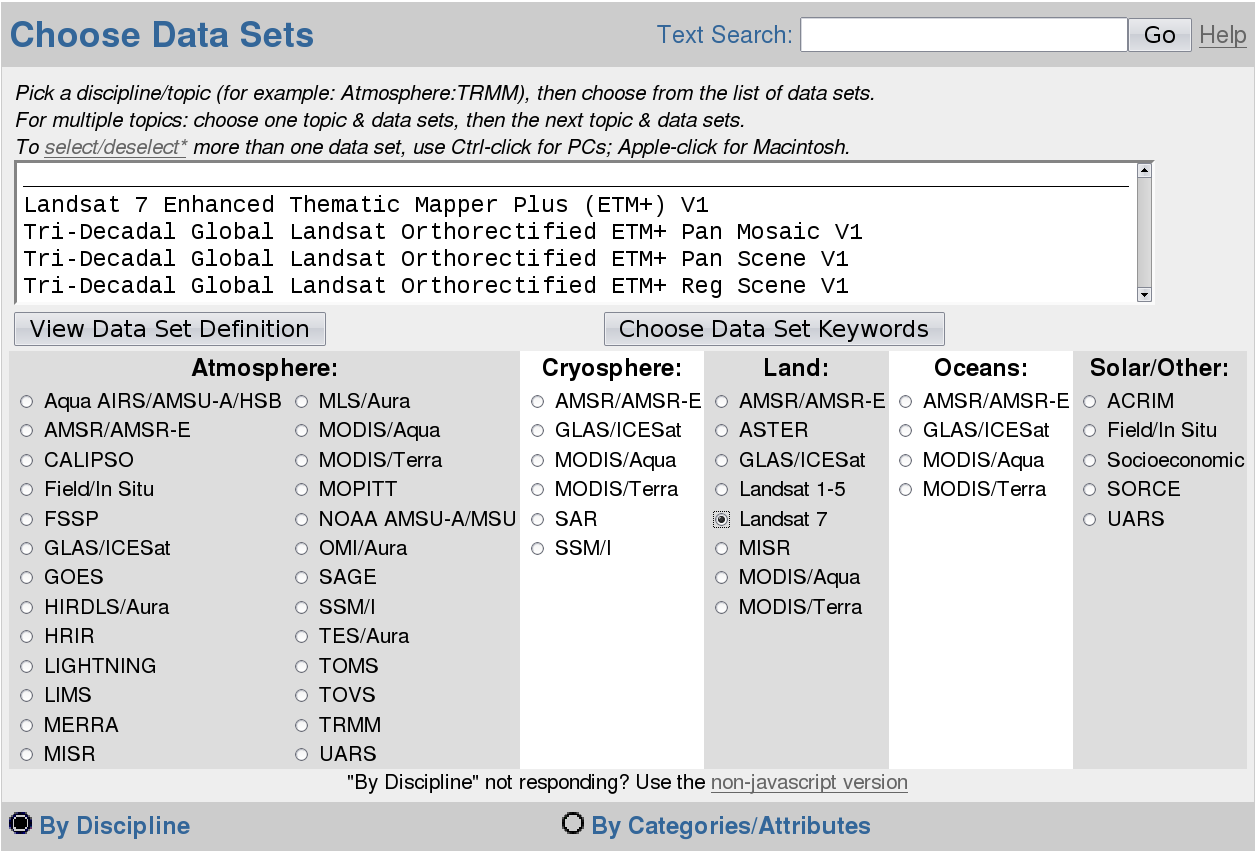
\includegraphics[scale=0.17]{WIST_datasets.png}
\end{center}
If you are downloading Modis images, be sure to have at hand a proper tool to manipulate the .hdf file format. The Modis Reprojection Tool (MRT) is such a tool and is available at (\href{http://lpdaac.usgs.gov/landdaac/tools/modis/index.asp}{lpdaac.usgs.gov/landdaac/tools/modis/}). MRT can convert to a more standard GeoTiff file format the Modis images. It can also reproject them to more common projection systems than its storage-purpose projection system the Integrated Sinusoidal. Alternatively, you can use a combination of tools from GDAL.\newline\linebreak
GDAL has a set of small tools that are practical to access information from header file and to perform repeated information on a dataset. You can use gdalinfo (\href{http://www.gdal.org/gdalinfo.html}{www.gdal.org/gdalinfo.html}) for extracting detailed information from the image file header, it extracts proper information about MODIS subdatasets and their naming conventions, add to it gdal\_translate (\href{http://www.gdal.org/gdal\_translate.html}{www.gdal.org/gdal\_translate.html}) to extract specific bands from the HDF format file into single bands common formats like GeoTiff. The script below automatically reads and exports each subdataset of any MODIS HDF file in the directory into a subdirectory called \textit{processed}.\newline
\begin{smallverbatim}
#This Unix Shell script automatically 
# extracts MODIS subdatasets into 
# processed/ subdirectory as GeoTiff 
# (*.tif) files
#-------------------------------------
mkdir processed
for file in *.hdf
do SDS_list=$(gdalinfo $file \
        | grep "SUBDATASET_.*_NAME.*")
	for subdataset in $SDS_list
	do echo ${subdataset#*=}.tif
	   gdal_translate -of GTiff \
	      ${subdataset#*=} processed/ \
	      ${subdataset#*=}.tif
	done
done
\end{smallverbatim}
Another tool, gdalwarp (\href{http://www.gdal.org/gdalwarp.html}{www.gdal.org/gdalwarp.html}) is dedicated to extract part of images and geolocate them properly. It would reproject the image data, it is useful to note that it also change the file format if you request it to do so. The script below does that with a target projection \textit{EPSG:4326} which actually means the following proj4 crs: \textit{+proj=longlat +ellps=WGS84 +datum=WGS84 +no\_defs}.
\begin{smallverbatim}
#This Unix Shell script automatically 
# extracts and reprojects MODIS 
# subdatasets into processed/ 
# subdirectory as GeoTiff (*.tif) files
#--------------------------------------
for file in *.hdf
do SDS_list=$(gdalinfo $file \
        | grep "SUBDATASET_.*_NAME.*")
	for subdataset in $SDS_list
	do echo ${subdataset#*=}.tif
	   gdalwarp -of GTiff \
	      -s_srs '+proj=sinu +R=6371007.181 \
	      +nadgrids=@null +wktext' \
	      -t_srs EPSG:4326 ${subdataset#*=} \
              processed/${subdataset#*=}.tif
	done
done
\end{smallverbatim}

\section{Renaming}
Most of the time you will want to reduce the size of the MODIS file names. As an example for MOD13Q1 NDVI layer renaming when converting from HDF to TIF, write the following script at the GRASS Command Line Interface:

\begin{smallverbatim}
#This Unix Shell script automatically 
# extracts MODIS NDVI subdatasets into 
# GeoTiff (*.tif) files with a sed 
# renaming scheme.
#-------------------------------------
root=~/MOD13Q1/2_PreProcessed
rootNDVI=$root/NDVI/
for file in MOD13Q1.A2010*.hdf
do 
	SDS_list_NDVI=$(gdalinfo $file \
		| grep "SUBDATASET_1_NAME")
	echo $file
	gdal_translate -of GTiff "${SDS_list_NDVI#*=}" \
	   $rootNDVI/$(echo ${SDS_list_NDVI#*=} \
	   | sed 's/\(.*\):\(.*\):"\(.*\).A\(.*\)\.\h \
	   \(.*\)\.\(.*\)\.\(.*\).hdf":\(.*\): \
	   \(.*\)/\3\_\4\_h\5\_\8\_250m_16_days_NDVI.tif/')
done
\end{smallverbatim}

If the later part of the code above is confusing, it may be a good idea to read about \href{http://www.gnu.org/software/sed/manual/sed.html}{sed} syntax.

\section{Importing in GRASS}
Once your files are prepared, they can be imported in GRASS.

\begin{smallverbatim}
#Import all NDVI files in a directory
# into GRASS GIS
#--------------------------------
cd $rootNDVI
for file in $rootNDVI
do
	r.in.gdal input=$file output=$file
done
\end{smallverbatim}

To access blindly an NDVI set of files, create a variable list from g.mlist:
\begin{smallverbatim}
#Create a list of NDVI files available
# in the current GRASS GIS Mapset
#-------------------------------------
listNDVI=$(g.mlist type=rast pattern=*NDVI*)
echo $listNDVI
\end{smallverbatim}

\section{QA Flags screening}
Use the \textit{i.modis.qc} module with MODIS Vegetation products (i.e. MOD13A2) as shown in the screenshot below:
\begin{smallverbatim}
MOD13A2: Mandatory QA Flags 1Km bits[0-1]
* [00]= class 0: VI produced, good quality
* [01]= class 1: VI produced, but check other QA
* [10]= class 2: Pixel produced, but most probably cloud
* [11]= class 3: Pixel not produced due to other \
    reasons than clouds
\end{smallverbatim}

\begin{center}
 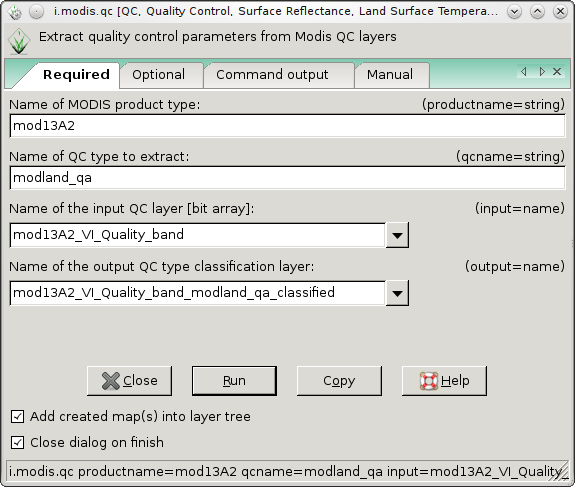
\includegraphics[scale=0.45]{i_modis_qc.png}
\end{center}

If you want to use shell scripting, the example below shows how to process Quality Assessment for Land Surface Temperature (i.e. MOD11A1):
\begin{smallverbatim}

MOD11A1: Mandatory QA Flags bits=[0-1]
* [00]= class 0: LST produced, good quality, \
    not necessary to examine more detailed QA
* [01]= class 1: LST produced, other quality, \
    recommend examination of more detailed QA
* [10]= class 2: LST not produced due to cloud effects
* [11]= class 3: LST not produced primarily due \
    to reasons other than cloud

for QC in mandatory_qa_11A1 data_quality_flag_11A1 \
 emis_error_11A1 lst_error_11A1
 do
 i.modis.qc productname=mod11A1 qcname=$QC \
 input=mod11A1.QC out=mod11A1_$QC
done
\end{smallverbatim}


\address{GRASS Development Team\\
  \url{http://grass.osgeo.org}\\
  \email{tmitchell@osgeo.org}}

%%% Local Variables: 
%%% mode: latex
%%% TeX-master: main\_document.tex
%%% End: 

